%start preamble
\documentclass[paper=a4,fontsize=11pt]{scrartcl}%kind of doc, font size, paper size

\usepackage{fontspec}
\defaultfontfeatures{Ligatures=TeX}
%\setsansfont{Liberation Sans}
\usepackage{polyglossia}	
\setdefaultlanguage[spelling=new, babelshorthands=true]{german}

\usepackage{amsmath}%get math done
\usepackage{amsthm}%get theorems and proofs done
\usepackage{graphicx}%get pictures & graphics done
\graphicspath{{pictures/}}%folder to stash all kind of pictures etc
\usepackage{amssymb}%symbolics for math
\usepackage{amsfonts}%extra fonts
\usepackage{caption}%captions under everything
\usepackage{listings}
\usepackage[titletoc]{appendix}
\numberwithin{equation}{section} 
\usepackage{float}%for garphics and how to let them floating around in the doc
\usepackage{wrapfig}%making graphics floated by text and not done by minipage
\usepackage{hyperref}
\usepackage{fancyhdr}
\usepackage{menukeys}
\usepackage{xcolor}%nicer colors, here used for links
\usepackage{csquotes}

\usepackage[backend=biber,style=alphabetic,
citestyle=alphabetic]{biblatex} %biblatex mit biber laden
\addbibresource{sources.bib}

%settings colors for links
\hypersetup{
    colorlinks,
    linkcolor={blue!50!black},
    citecolor={blue},
    urlcolor={blue!80!black}
}

\definecolor{pblue}{rgb}{0.13,0.13,1}
\definecolor{pgreen}{rgb}{0,0.5,0}
\definecolor{pred}{rgb}{0.9,0,0}
\definecolor{pgrey}{rgb}{0.46,0.45,0.48}

\pagestyle{fancy}
\lhead{Netzwerke Übung (SoSe 2020)}
\rhead{FB 4 -- Angewandte Informatik\\ HTW-Berlin}
\lfoot{Übungsblatt 04 -- Wireshark}
\cfoot{}
\fancyfoot[R]{\thepage}
\renewcommand{\headrulewidth}{0.4pt}
\renewcommand{\footrulewidth}{0.4pt}

\lstdefinestyle{Bash}{
  language=bash,
  showstringspaces=false,
  basicstyle=\small\sffamily,
  numbers=left,
  numberstyle=\tiny,
  numbersep=5pt,
  frame=trlb,
  columns=fullflexible,
  backgroundcolor=\color{gray!20},
  linewidth=0.9\linewidth,
  %xleftmargin=0.5\linewidth
}

%%here begins the actual document%%
\newcommand{\horrule}[1]{\rule{\linewidth}{#1}} % Create horizontal rule command with 1 argument of height

\DeclareMathOperator{\id}{id}

\begin{document}
\begin{center}
\Large{\textbf{Übungsblatt 4 -- Wireshark}}
\end{center}

\begin{center}\Large{\textbf{Aufgabe A -- OSI-Modell \& Transport Layer + IP}}\end{center}\vskip0.25in
Da Sie in der kommenden Übung mithilfe \emph{Wiresharks} Ihren Netzwerkverkehr untersuchen sollen, müssen Sie zumindest grundlegend verstanden haben auf welche Protokolle Sie dort stoßen werden.
\begin{enumerate}
	\item Schauen Sie folgendes Video: \url{https://youtu.be/iDCi_CJAyXs} (Transport Layer)
	\item Recherchieren Sie die Funktion, sowie den Aufbau des \emph{TCP}-Protokolls.\\
	\url{https://youtu.be/_WP9be9W3xE}
	\begin{enumerate}
		\item Auf welcher Ebene im OSI-Modell arbeitet \emph{TCP}?
		\item Welche Aufgabe übernimmt das oben genannte Protokoll?
		\item Aus welchen Segmenten besteht ein \emph{TCP}-Datagram?
		\item Zeigen Sie beispielhaft den Aufbau eines \emph{TCP}-Datagram.
	\end{enumerate}
	\item Recherchieren Sie die Funktion, sowie den Aufbau des \emph{UDP}-Protokolls.\\
	\url{https://youtu.be/xWsD6a3KsAI}
	\begin{enumerate}
		\item Auf welcher Ebene im OSI-Modell arbeitet \emph{UDP}?
		\item Welche Aufgabe übernimmt das oben genannte Protokoll?
		\item Aus welchen Segmenten besteht ein \emph{UDP}-Datagram?
		\item Zeigen Sie beispielhaft den Aufbau eines \emph{UDP}-Datagram.
	\end{enumerate}
	\item Worin unterscheiden sich \emph{TCP} und \emph{UDP} grundlegend?
	\item Recherchieren Sie die Funktion, sowie den Aufbau des IP-Protokolls.
	\begin{enumerate}
		\item Auf welcher Ebene im OSI-Modell arbeitet IP?
		\item Welche Aufgabe übernimmt das oben genannte Protokoll?
		\item Aus welchen Segmenten besteht ein IP-Paket im allgemeinen?
	\end{enumerate}
	\item Recherchieren Sie die Funktion, sowie den Aufbau von Ethernet (\emph{IEEE 802.3} Protokollfamilie).
	\begin{enumerate}
		\item Auf welcher Ebene im OSI-Modell arbeitet \emph{Ethernet}?
		\item Welche Aufgabe übernimmt das oben genannte Protokoll?
		\item Aus welchen Segmenten besteht ein Ethernet-Frame?
	\end{enumerate}	
\end{enumerate}

\begin{center}\Large{\textbf{Aufgabe B -- TCP: 3-Way-Handshake}}\end{center}\vskip0.2in
Da TCP ein verbindungsorientiertes Protokoll ist, ist der Aufbau eines Sockets etwas komplizierter. Beide Seiten müssen sichergehen, dass die Verbindung korrekt funktioniert.
\begin{enumerate}
	\item Recherchieren Sie wie der 3-Way-Handshake bei TCP funktioniert \citep[S. 252f]{Kurose2012}
	\item Gegeben sei Folgendes Sequenzdiagramm einer TCP Verbindung.
	\begin{figure}[H]
		\centering
		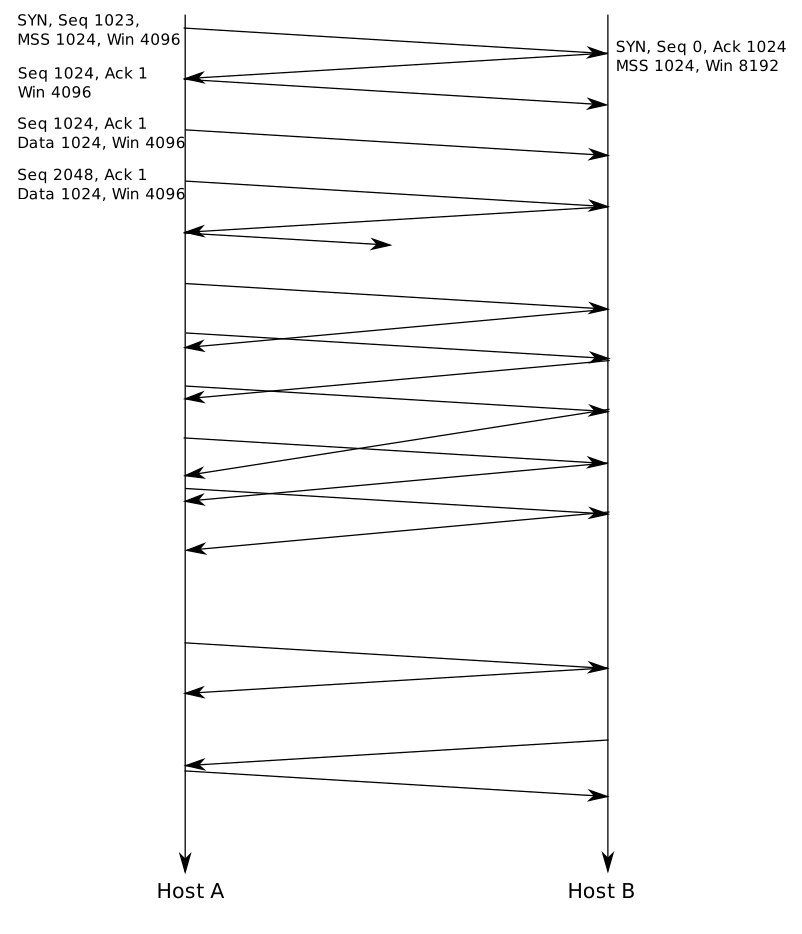
\includegraphics[scale=0.3]{handshake}
	\end{figure}
	Die horizontalen Pfeile repräsentieren die Zeit. Die Beschriftungen sollen die Header-Felder der TCP-Segmente beschreiben. Eine 3-Way-Handshake wird von Host A initialisiert.
	\item Erläutern Sie den Austausch der ersten drei Segmente und Werte der Header-Felder.
	\item Host $A$ übermittelt 7 Segmente mit einer Nutzlast (Payload) von 1024 Byte an Host $B$, anschließend schließt $A$ die Verbindung. Die ersten beiden Segmente samt Nutzdaten sind im Sequenzdiagramm bereits beschriftet. Vervollständigen Sie die restlichen Segmente samt Werte anhand folgender Informationen:
	\begin{itemize}
		\item[a)] Eines der Segmente ging verloren (signalisiert durch eine Pfeil der nicht die rechte Seite erreicht)
		\item[b)] Nehmen Sie an, das Host $A$ den Fast-Retransmit unterstützt und keine Timeouts durch ein verlorenes Segment auftritt.
	\end{itemize}
\end{enumerate}

\begin{center}\Large{\textbf{Aufgabe C -- ICMP}}\end{center}\vskip0.2in
Bevor es zum Thema Routing geht, soll im Folgenden noch das ICM-Protokoll betrachtet werden. Dieses dient in vielen Fällen als Diagnoseprotokoll.
\begin{enumerate}
	\item Lesen Sie den Abschnitt 4.4.3 zu ICMP \cite[S. 353]{Kurose2012}. 
	\item Was ist die Funktion des Internet Control Message Protocol (ICMP)?
	\item ICMP hat verschiedene Message-Codes (einige brauchen wir in den Übungen 4 und 5!). Erläutern Sie was diese Nachrichten kodieren sollen -- was ist der Zweck der Message-Codes?
	\item Recherchieren Sie welchen Hinweis Ihnen die verschiedenen \emph{ICMP}-Messages geben.
		\begin{itemize}
			\item[i)] Echo
			\item[ii)] Echo Reply
		\end{itemize}
\end{enumerate}

\begin{center}\Large{\textbf{Aufgabe D -- Routing}}\end{center}\vskip0.2in
\begin{enumerate}
	\item Im wesentlichen gibt es zwei fundamentale Routing-Algorithmen. Dies sind das Distanz-Vektor- und Link-State-Routing. Diese ermöglichen es den kürzesten Weg durch einen Graphen zu finden (Shortest-Path-Problem).\\
	Für gewöhnlich wird für das Distanz-Vektor-Routing der Bellman-Ford-Algorithmus verwandt, das Link-State-Routing nutzt den Dijkstra-Algorithmus. \cite[S. 363ff]{Kurose2012}
	\begin{enumerate}
		\item Recherchieren Sie wie das Link-State-Routing unter Nutzung des Dijkstra-Algorithmus funktioniert \cite[S. 366]{Kurose2012}.
		\item Recherchieren Sie wie das Distanz-Vektor-Routing unter Nutzung des Bellman-Ford-Algorithmus funktioniert  \cite[S. 371]{Kurose2012}.
		\item In welchen Protokollen finden diese beiden Protokollen Verwendung? Ist diesen Protokollen etwas gemein?
		\item Erläutern Sie die fundamentalen Unterschiede beider Lösungsansätze.
		\item Warum wird keines der beiden Verfahren für das Exterior-Gateway-Protokoll (EGP) genutzt?
		\item Diskutieren Sie ob der Bellman-Ford-Algorithmus für das Link-State-Routing und der Dijkstra-Algorithmus für das Distanz-Vektor-Routing genutzt werden könnte.
	\end{enumerate}
	\item Gegeben sei folgender Graph:
	\begin{figure}[H]
		\centering
		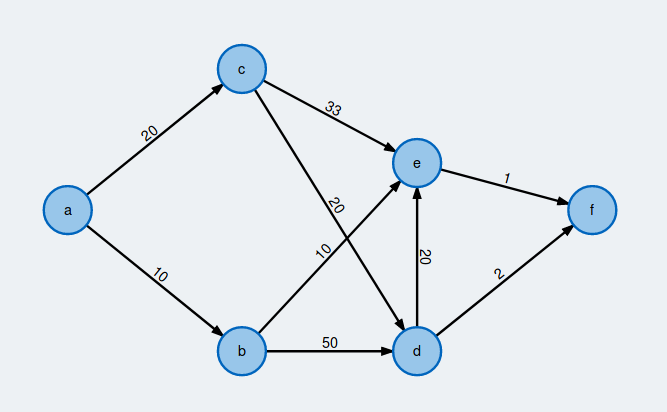
\includegraphics[scale=0.4]{dijkstra_example}
	\end{figure}
	Finden Sie den kürzesten Weg vom Knoten $a$ zum Knoten $f$!
	\begin{enumerate}
		\item Nutzen Sie zunächst den Dijkstra-Algorithmus.
		\item Nutzen Sie den Bellman-Ford-Algorithmus.
	\end{enumerate}
\end{enumerate}

\begin{center}\Large{\textbf{Aufgabe E -- Traceroute}}\end{center}\vskip0.2in
\begin{enumerate}
	\item Lesen Sie die folgenden Artikel:\\
	\url{https://en.wikipedia.org/wiki/Traceroute},\\
	\url{https://linux.die.net/man/8/traceroute}.\\
	Beantworten Sie anschließend folgende Fragen:
	\begin{enumerate}
		\item Wofür wird Traceroute genutzt?
		\item Wie wird Traceroute umgesetzt, d.h. wie läuft eine \enquote{Routen-Verfolgung} ab? 
		\item Welche ICMP-Messages werden für die Realisierung genutzt?
		\item Welche Limitationen ergeben sich aus dieser Umsetzung?
		\item Dokumentieren Sie die Syntax, sowie die Bedeutung von Traceroute beispielhaft.
	\end{enumerate}
	\item Lesen Sie folgendes Paper zu Paris-Traceroute \cite{Augustin2006ATA} von der ACM International Measurement Conference (IMC) 2006:\\
	\url{http://conferences.sigcomm.org/imc/2006/papers/p15-augustin.pdf}
	\begin{enumerate}
		\item Warum ist eine \enquote{neue} Traceroute-Applikation notwendig?
		\item Nennen Sie drei Topologie-Anomalien die durch Paris-Traceroute erkannt werden kann.
		\item Recherchieren Sie wie \emph{paris-traceroute} zu nutzen ist! Notieren Sie sich entsprechend die Kommandos und deren Bedeutung.
	\end{enumerate}
\end{enumerate}
\printbibliography
\end{document}


